In questo capitolo verrà affrontata la generazione del grafo di scena dato un frame e l'aggiornamento della Mappa Semantica con queste nuove informazioni per manterla aggiornata rispetto all'ambiente.
\begin{figure}[h]
	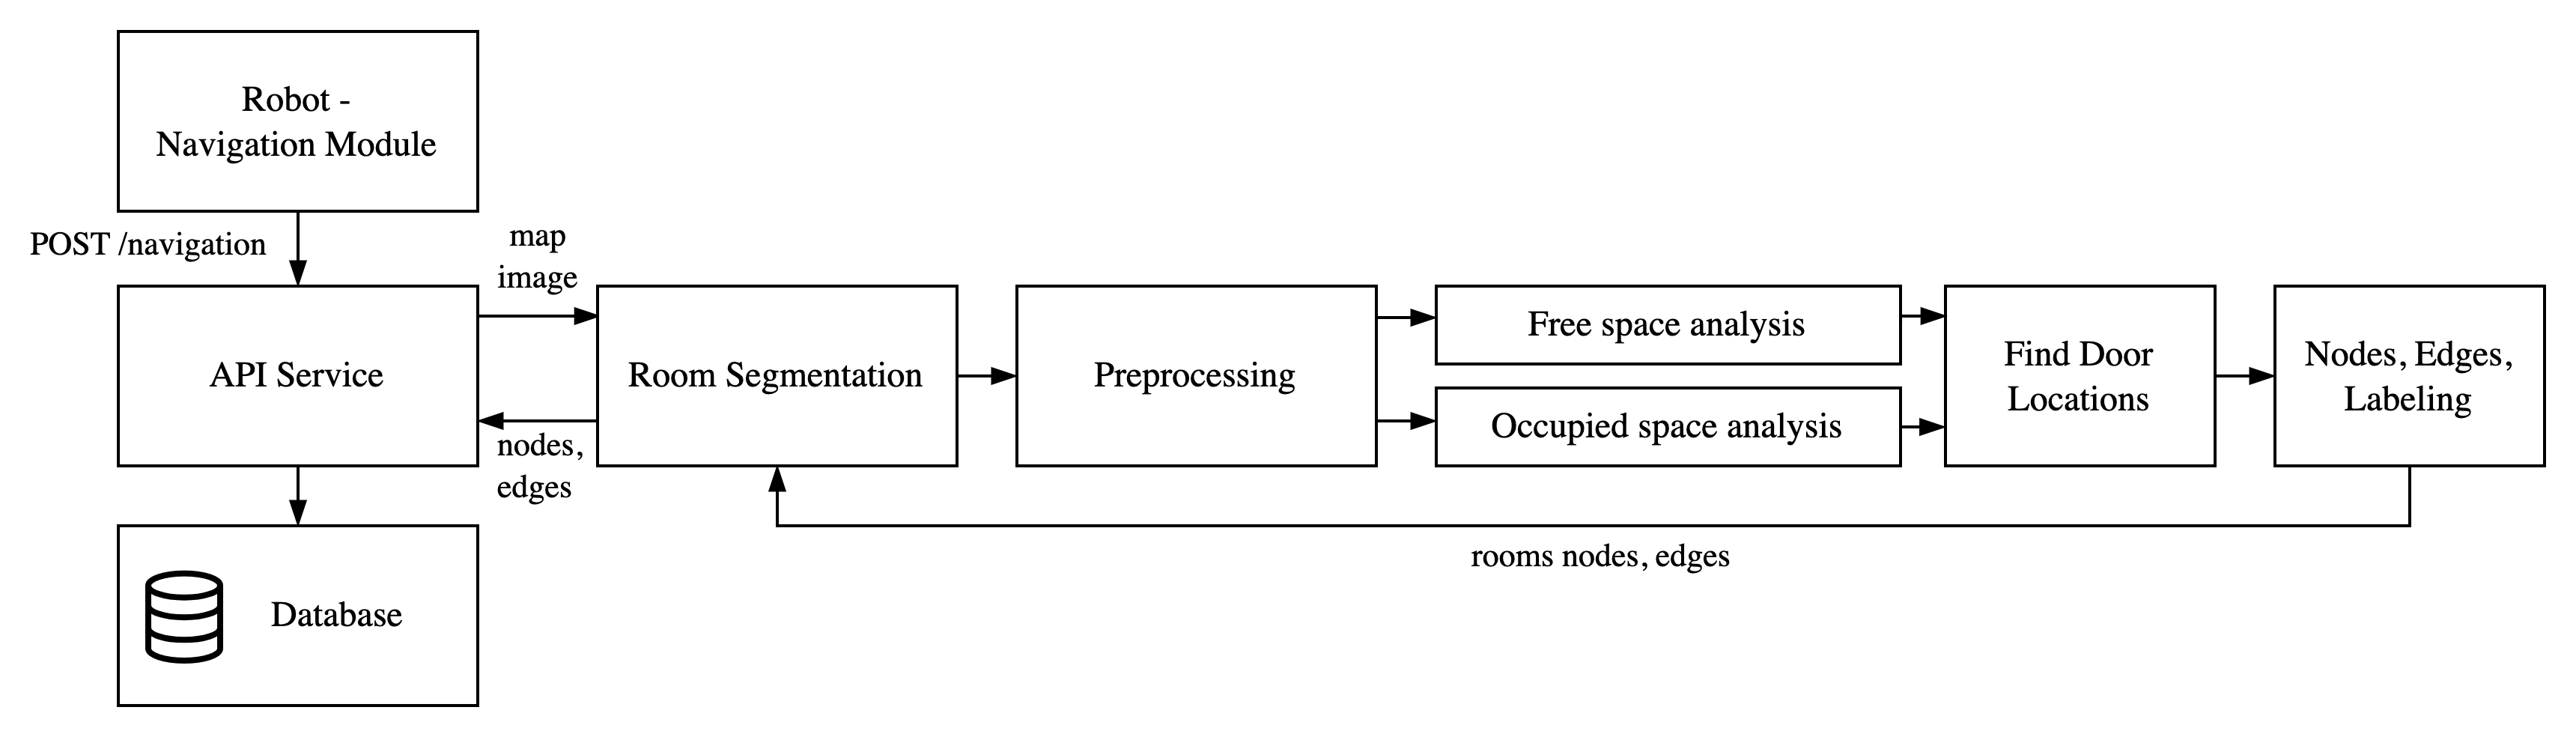
\includegraphics[width=\textwidth]{scene_graph/general_data_flow.png}
	\caption{Schema dei flussi dati per la generazione del grafo di scena e aggiornamento della mappa semantica }
\end{figure}

\section{Generazione del Grafo di Scena}
La generazione del grafo di scena è un passo fondamentale per il mantenimento della coerenza tra Mappa Semantica e Ambiente reale.\\
Il grafo di scena è una struttura dati che rappresenta gli oggetti presenti nell'ambiente e le relazioni tra loro composto da nodi e archi. I nodi rappresentano gli oggetti, mentre gli archi rappresentano le relazioni tra gli oggetti. \\
In questa sezione verrà affrontata la costruzione di questa struttura dati a partire da un frame RGB-D e il modello di ML utilizzato per l'inferenza degli oggetti e delle relazioni.
\subsection{Lettura del frame RGB-D}
All'interno dell'architettura cloud-native di Robee vi è la presenza di un pod chiamato "Streaming Module" il cui compito è streammare il feed video delle camera sul pod redis del robot, in modo che gli altri servizi o moduli possano accedere a questi dati tramite l'utilizzo di librerie wrapper, rendendo il tutto agnostico rispetto alla tipologia e al modello di videocamera utilizzati.

\subsection{Inferenza}
Ogni frame ricevuto dal feed video viene successivamente dato in input al modello PSGTr \cite{yang2022psg} che restituisce un oggetto di tipo Detections il quale contiene i seguenti dati:
\begin{itemize}
	\item labels: lista con lunghezza pari al numero di oggetti rilevati. Ogni valore indica la label corrispondente all' $i$-esimo oggetto. Per esempio, l'oggetto $i$-esimo ha label $labels[i]$;
	\item masks: lista contenente le maschere di ogni oggetto rilevato;
	\item bboxes: lista contenente le bounding boxes di ogni oggetto rilevato;
	\item rel\_pair\_idxes: lista con lunghezza pari al numero di relazioni tra oggetti rilevate. Ogni valore è a sua volta un array di dimensione due contenente gli indici dell'oggetto target e dell'oggetto sorgente della relazione;
	\item rel\_labels: lista con lunghezza pari al numero di relazioni tra oggetti rilevate. Ogni valore indica la label della $i$-esima relazione
	\item rel\_dists: lista con lunghezza pari al numero di relazioni tra oggetti rilevate. Ogni valore indica la probabilità associata alla $i$-esima relazione.
\end{itemize}
Questi dati vengono successivamente utilizzati per la costruzione del grafo di scena.

\subsubsection{Panoptic Scene Graph - Transformer}
Il modello PSGTr \cite{yang2022psg} è un modello di deep learning a singolo stato basato su architettura Transformer \cite{transformer} il cui obiettivo è quello di generare una rappresentazione a grafo della scena data la segmentazione panottica piuttosto che le bounding box degli oggetti rilevati.
\paragraph*{Training}
Il modello, per quanto riguarda gli oggetti, è stato addestrato su un dataset composto da 49mila immagini annotate basato su COCO \cite{coco} e Visual Genome \cite{visualgenemo}. Per le relazioni hanno estratto e costruito un dataset di 56 predicati a partire da dataset come VG-150 \cite{vg150}, VrR-VG \cite{vrvvg} and GQA \cite{cqa}.
\paragraph*{Segmentazione Panoptica}
La segmentazione panoptica individua gli oggetti e assegna a ogni pixel la label della classe dell'oggetto a cui appartengono. L'utilizzo di questa rispetto alle bounding da notevoli vantaggi:
\begin{itemize}
	\item Garantisce una localizzazione più precisa degli oggetti, segmentandoli a livello di pixel e riducendo la presenza di pixel rumorosi o ambigui tipici delle bounding box, che spesso includono porzioni di altre categorie o oggetti;
	\item Copre l'intera scena di un'immagine, inclusi gli sfondi, offrendo una comprensione più completa del contesto rispetto alle bounding box, che tendono a trascurare importanti informazioni di sfondo;
	\item Riduce anche le informazioni ridondanti o irrilevanti presenti nei dataset basati su bounding box, focalizzandosi sulla segmentazione degli oggetti piuttosto che sulle loro parti.
\end{itemize}
\paragraph*{Funzionamento di PSGTr}
L'architettura di PSGTr è basata su DETR \cite{detr} e HOI \cite{hoi}. Il modello predice triple $(soggetto, predicato, verbo)$ e la localizzazione degli oggetti simultaneamente.
\paragraph*{Pipeline PSGTr}
Attraverso una \gls{backbone} CNN, PSGTr estrae le features dell'immagine e i positional encodings che, insieme alle triplet queries, vengono dati in input al transformer encoder-decoder. In questo processo, l'obiettivo è che le query apprendano la rappresentazione del grafo di scena a triple in modo che per ognuna di esse, le predictions di  $(soggetto, predicato, verbo)$ possano successivamente essere estratte da tre Feed Forward Network. Infine, il task di segmentazione viene eseguito da due head panoptiche, una per il soggetto e una per l'oggetto della relazione.

\subsection{Costruzione del grafo}
L'obiettivo di questo step è la costruzione del grafo di scena rispetto all'ultimo frame. Per farlo, è necessario estrarre i dati dai risultati dell'inferenza di PSGTr e calcolare quei valori che dipendono dal sistema robot, come la posizione.
L'algoritmo di costruzione del grafo è costituito da 2 fasi principali:
\begin{itemize}
	\item Costruzione dei nodi per la scena semantica e per la mappa semantica:
	      \begin{itemize}
		      \item Calcolo della posizione dell'oggetto
	      \end{itemize}
	\item Costruzione degli archi per la scena semantica e per la mappa semantica
\end{itemize}

\subsubsection{Costruzione dei nodi}
\paragraph{Estrazione dati oggetto dai risultati}
L'oggetto MMDetResult ritornato dalla funzione di inferenza del modello, come detto precedentemente, possiede un attributo $labels$ che è una lista con lunghezza pari al numero di oggetti rilevati dove il valore $i$-esimo, indica l'indice della classe di appartenenza dell'oggetto $i$. Lo stesso meccanismo vale anche per le maschere.

\begin{algorithm}
	\caption{Estrazione classi e maschere degli oggetti individuati}
	\begin{algorithmic}[1]
		\State $obj\_classes \gets \text{[ ]}$
		\State $obj\_masks \gets \text{[ ]}$
		\State $obj\_labels\_ids \gets detectionResults.labels$
		\For{ $i=0$ to $obj\_labels\_ids.length$}
		\State $obj\_classes.append(PSG\_CLASSES[obj\_labels\_ids[i]])$
		\State $obj\_masks.append(detectionResults.masks[i])$
		\EndFor
	\end{algorithmic}
\end{algorithm}


\paragraph{Calcolo posizioni 3D}
Per ogni oggetto, si estrae la posizione 3D nella mappa del robot in modo che questo possa successivamente localizzarlo e raggiungerlo.
\subparagraph{Calcolo posizione 3D nel \gls{pixel_system}}
Le maschere generate dal modello consentono di calcolare il centroide $(x_i, y_i)$ dell'oggetto $i$-esimo. Tuttavia, queste maschere forniscono solo un valore in due dimensioni. Per il calcolo del valore $z_i$ si utilizza il \Gls{point_cloud} che, combinando il frame RGB con il frame Depth, permette di ottenere una rappresentazione 3D della scena. \\
Per ogni oggetto $i$, si maschera il Point Cloud con la maschera $i$-esima e si calcola $z_i$ come valore mediano tra le $z_s$ di tutti i punti mascherati ottenendo cosí una posizione $P_{ipd} = (x_i, y_i, z_i)$.
% Reference System Image with panoptic example
\begin{figure}[h]
	\tdplotsetmaincoords{-10}{0}
	\begin{tikzpicture}[tdplot_main_coords]
		\begin{scope}[canvas is xy plane at z=0]
			\node[anchor=north west, inner sep=0] at (0,0) {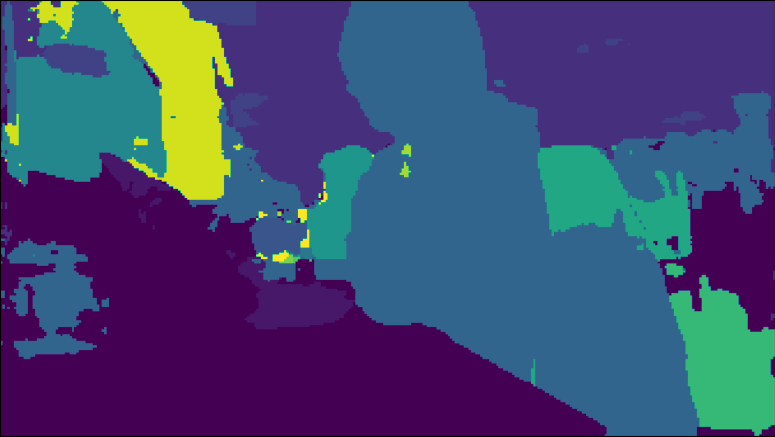
\includegraphics[width=4cm]{scene_graph/segmentation_labeling.png}};
		\end{scope}

		% Draw the x-axis vector
		\draw[->, thick, red] (0,0,0) -- (3,0,0) node[anchor=north east]{$\mathbf{x}$};

		% Draw the y-axis vector
		\draw[->, thick, green] (0,0,0) -- (0,-2.8,0) node[anchor=north west]{$\mathbf{y}$};

		% Draw the z-axis vector
		\draw[->, thick, blue] (0,0,0) -- (1,0.5,-3) node[anchor=south]{$\mathbf{z}$};

		% Add labels for the origin
		\node at (0,0.4,0) [below left] {O};
	\end{tikzpicture}
	\caption{Sistema di coordinate pixel}
\end{figure}

\begin{algorithm}
	\caption{Calcolo della posizione 3D nel sistema pixel}
	\begin{algorithmic}[1]
		\Procedure{get\_pixel\_coords}{depth\_frame, obj\_mask}
		\State $z_{ip} \gets \text{median}(depth\_frame[obj\_mask])$ \Comment{Point Cloud}
		\State $x_{ip} \gets \text{median}(obj\_mask[:, 0])$
		\State $y_{ip} \gets \text{median}(obj\_mask[:, 1])$
		\State \Return $x_{ip}, y_{ip}, z_{ip}$
		\EndProcedure
	\end{algorithmic}
\end{algorithm}

\subparagraph{Calcolo posizione 3D nel \gls{camera_system}}
Per ogni oggetto $i$, è necessario trasformare la posizione $P_{ipd}$ nel sistema di coordinate della camera, ovvero con la camera nell'origine. A tale scopo, si utilizza la \textbf{Matrice Intrinseca della Camera} ovvero la \gls{homogeneous_transformation_matrix} usata per convertire le coordinate in sistema camera a coordinate in sistema pixel. Questa dipende da caratteristiche fisiche della camera come apertura focale, campo visivo e risoluzione.\\
Poichè è necessario eseguire il procedimento inverso, ovvero trasformare le coordinate $P_{ipd}$ in sistema pixel a coordinate in sistema camera, viene utilizzata la Matrice Instrinseca Inversa e si esegue il prodotto matriciale tra questa e le coordinate $P_{ipd}$ aumentate, ottenendo così la posizione $P_{ic}$ degli oggetti in sistema camera.

\[
	\begin{bmatrix}
		x_{ic} \\
		y_{ic} \\
		z_{ic} \\
		1
	\end{bmatrix}
	=
	M_{ic}^{-1}
	*
	\begin{bmatrix}
		x_{ip} \\
		y_{ip} \\
		z_{ip} \\
		1
	\end{bmatrix}
\]

Dove:
\begin{itemize}
	\item $M_{ic}$ è la Matrice Intrinseca della Camera
	\item $x_{ip}, y_{ip}, z_{ip}$ sono le coordinate in sistema pixel dell'oggetto $i$
	\item $x_{ic}, y_{ic}, z_{ic}$ sono le coordinate in sistema camera dell'oggetto $i$
\end{itemize}

\begin{figure}[h]
	\tdplotsetmaincoords{-10}{0}
	\begin{tikzpicture}[tdplot_main_coords]
		\begin{scope}[canvas is xy plane at z=0]
			\node[anchor=center, inner sep=0, fill=white] at (0,0) {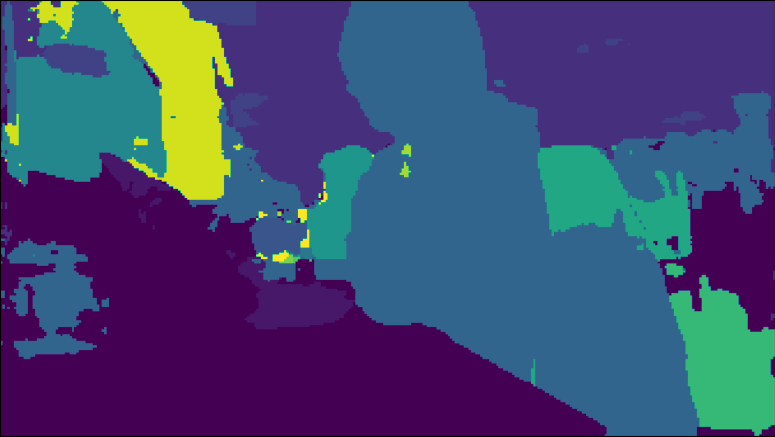
\includegraphics[width=4cm]{scene_graph/segmentation_labeling.png}};
		\end{scope}

		% Draw the x-axis vector
		\draw[->, thick, red] (0,0,0) -- (1,0.5,-2) node[anchor=south]{$\mathbf{x}$};

		% Draw the y-axis vector
		\draw[->, thick, green] (0,0,0) -- (-2, 0,0) node[anchor=north west]{$\mathbf{y}$};

		% Draw the z-axis vector
		\draw[->, thick, blue] (0,0,0) -- (0, 2, 0) node[anchor=south]{$\mathbf{z}$};

		% Add labels for the origin
		\node[] at (0,0.4,0) [below left] {\textcolor{white}{O}};
	\end{tikzpicture}
	\caption{Sistema di coordinate camera}
\end{figure}

\begin{algorithm}[h]
	\caption{Calcolo della posizione 3D nel sistema camera}
	\begin{algorithmic}[1]
		\Procedure{get\_camera\_coords}{$P_{ip}$}
		\State $M_{ic} \gets \Call{get\_camera\_intrinsics}{}$ \Comment{Funzione libreria Robee}
		\State $P_{ic} \gets M_{ic}^{-1} \times P_{ip}$
		\State $distance = norm(P_{ic} - P_{\text{camera}})$
		\State \Return $P_{ic}, distance$
		\EndProcedure
	\end{algorithmic}
\end{algorithm}

\subparagraph{Calcolo posizione 3D nel sistema mappa}
L'ultimo passaggio per ottenere la posizione dell'oggetto nella mappa è quello di utilizzare la Matrice Estrinseca della Camera, ovvero la \gls{homogeneous_transformation_matrix} usata per convertire le coordinate in sistema mondo a coordinate in sistema camera. Dipende dalla posizione e dall'orientamento della camera nel mondo. \\\\
Dato che in questo contesto la camera è montata sulla testa del robot, la matrice estrinseca dipende dalla posizione e dall'orientamento di quest'ultima e a seguire di tutte le trasformate nell'\gls{tf_tree} del robot. All'interno dell'architettura di Robee, sono presenti due moduli che si occupano di calcolare le trasformate per passare da un sistema di coordinate ad un altro. Si utilizzano dunque questi moduli per calcolare la matrice estrinseca inversa rispetto alla mappa/robot che moltiplicata per le coordinate $P_{ic}$ ottenute precedentemente, permette di ottenere la posizione dell'oggetto nel sistema mappa/robot.

\[
	\begin{bmatrix}
		x_{im} \\
		y_{im} \\
		z_{im} \\
		1
	\end{bmatrix}
	=
	M_{ec}^{-1}
	*
	\begin{bmatrix}
		x_{ic} \\
		y_{ic} \\
		z_{ic} \\
		1
	\end{bmatrix}
\]

Dove:
\begin{itemize}
	\item $M_{ec}$ è la Matrice Estrinseca della Camera
	\item $x_{ic}, y_{ic}, z_{ic}$ sono le coordinate in sistema camera dell'oggetto $i$
	\item $x_{im}, y_{im}, z_{im}$ sono le coordinate in sistema mappa dell'oggetto $i$
\end{itemize}

\begin{algorithm}
	\caption{Calcolo della posizione 3D nel sistema mappa}
	\begin{algorithmic}[1]
		\Procedure{get\_map\_coords}{$P_{ic}$}
		\State $M_{ec} \gets \Call{get\_camera\_extrinsics}{}$ \Comment{Funzione libreria Robee}
		\State $P_{im} \gets M_{ec}^{-1} \times P_{ic}$
		\State \Return $P_{im}$
		\EndProcedure
	\end{algorithmic}
\end{algorithm}

\paragraph{Istanziamento dei nodi}
Con tutti i dati ora a dispozione è possibile istanziare i nodi per la scena semantica e per la mappa semantica. Per la scena semantica, si istanziano i nodi con la posizione 3D nel sistema di riferimento del robot, mentre per la mappa semantica, si istanziano i nodi con la posizione 3D nel sistema di riferimento della mappa. \\
A causa del rumore del frame Depth nelle zone troppe vicine o troppo lontane dalla camera, è necessaria l'applicazione di un filtro per escludere gli oggetti che distano troppo dalla camera o che sono troppo vicini. Le soglie di distanza vengono impostate nei parametri di configurazione del servizio.

\begin{algorithm}
	\caption{Instanziamento dei nodi}
	\begin{algorithmic}[1]
		\State $obj\_ids \gets \text{[ ]}$
		\For{ $i=0$ to $obj\_labels\_ids.length$}
		\State $obj\_pixel\_coords \gets \Call{get\_pixel\_coords}{depth\_frame, obj\_masks[i]}$
		\State $obj\_camera\_coords, distance \gets \Call{get\_camera\_coords}{obj\_pixel\_coords}$
		\State $obj\_coords \gets \Call{get\_map\_coords}{obj\_camera\_coords}$
		\If{$distance > min\_distance$ \textbf{and} $distance < max\_distance$}
		\State $node \gets \text{Node}(i, obj\_classes[i], obj\_coords)$
		\State $obj\_ids.append(i)$
		\State $semantic\_scene.add\_node(node)$
		\State $semantic\_map.add\_node(node)$
		\EndIf
		\EndFor
	\end{algorithmic}
\end{algorithm}

\subsubsection{Costruzione degli archi}

\paragraph{Estrazione dati relazione dai risultati}
L'oggetto MMDetResult ritornato dalla funzione di inferenza del modello, come detto precedentemente, possiede gli attributi:
\begin{itemize}
	\item $rel\_labels$: lista con lunghezza pari al numero di relazione rilevate dove il valore $j$-esimo, indica l'indice della classe di appartenenza della relazione $j$.
	\item rel\_pair\_idxes: lista con lunghezza pari al numero di relazioni tra oggetti rilevate. Ogni valore è a sua volta un array di dimensione due contenente gli indici dell'oggetto target e dell'oggetto sorgente della relazione;
	\item $rel\_dist$: lista con lunghezza pari al numero di relazione rilevate dove il valore $j$-esimo, indica la probabilità associata alla relazione $j$.
\end{itemize}
È necessario estrarre questi dati e mettere in relazione gli oggetti tra loro per costruire gli archi del grafo.\\
Per ogni relazione $j$, si estrae l'indice dell'oggetto sorgente $s$ e l'indice dell'oggetto target $t$ e viene creato un arco tra i nodi corrispondenti se:
\begin{itemize}
	\item Entrambi i nodi siano presenti nella lista di oggetti precedentemente calcolata, ovvero rispettano i vincoli di distanza.
	\item La probabilità associata alla relazione sia maggiore di una certa soglia, impostata nei parametri di configurazione del servizio.
\end{itemize}

\begin{algorithm}
	\caption{Instanziamento degli archi}
	\begin{algorithmic}[1]
		\For{ $j=0$ to $rel\_labels.length$}
		\State $source\_idx \gets rel\_pair\_idxes[j][0]$
		\State $target\_idx \gets rel\_pair\_idxes[j][1]$
		\If{$source\_idx$ \textbf{in} $obj\_ids$ \textbf{and} $target\_idx$ \textbf{in} $obj\_ids$}
		\State $source\_node \gets semantic\_scene.get\_node(source\_idx)$
		\State $target\_node \gets semantic\_scene.get\_node(target\_idx)$
		\If{$rel\_dist[j] > rel\_threshold$}
		\State $semantic\_scene.add\_edge(source\_node, target\_node, rel\_labels[j])$
		\EndIf
		\EndIf
		\EndFor
	\end{algorithmic}
\end{algorithm}

\section{Aggiormento del Mappa Semantica}
In questa sezione verrà affrontato il processo di aggiornamento della Mappa Semantica con i nuovi dati ottenuti dalla Generazione del Grafo di Scena della sezione precedente.\\
La Mappa Semantica è una struttura dati che rappresenta l'ambiente circostante il robot e che viene aggiornata in real time per mantenere la coerenza con l'ambiente reale.\\
Il processo di aggiornamento della Mappa Semantica è composto da 3 fasi principali:
\begin{itemize}
	\item Trovare la stanza corrente del robot utilizzando il Grafo delle Stanze della Mappa Semantica
	\item Aggiornare il Grafo degli Oggetti della stanza corrente con i nuovi nodi e archi.
	\item Aggiornare la Mappa Semantica su DB e pubblicare i nuovi risultati sul relativo topic MQTT.
\end{itemize}

\subsection{Trovare la stanza corrente del robot}
Trovare la stanza corrente del robot è uno step necessario: permette di aggiornare il Grafo degli Oggetti della sola la stanza in cui il robot si trova, evitando di aggiornare l'intera mappa, efficientando il processo.\\
% is_inside_polygon
\subsubsection{Algoritmo di Ray Casting}
Ogni nodo stanza della Mappa Semantica ha un attributo $segments$ che rappresenta i segmenti che delineano i confini della stanza fisica. \\
Per determinare la stanza in cui si trova il robot, si utilizza l'algoritmo di Ray Casting \cite{haines_199424} che permette di determinare se un punto è all'interno di un poligono, il cui funzionamento è il seguente:
\begin{itemize}
	\item Si sceglie come punto di inizio $P_{start}$ del raggio un punto che sicuramente è all'esterno del poligono.
	\item Si emette un raggio dal punto $P_{start}$ al punto $P_{check}$ che si vuole verificare se è all'interno del poligono.
	\item Si contano quante volte il raggio interseca i segmenti del poligono:
	      \begin{itemize}
		      \item Se il numero è dispari, il punto è all'interno del poligono;
		      \item Se il numero è pari, il punto è all'esterno del poligono.
	      \end{itemize}
\end{itemize}
L'intuizione alla base di questo algoritmo è che se il segmento che congiunge il punto esterno e il punto $P_{check}$ interseca un numero dispari di segmenti del poligono significa che ho incontrato solo un "bordo" del poligono e quindi il punto è all'interno. Se il numero è pari, significa che ho incontrato due "bordi" e quindi sono o entrato e poi uscito dal poligono oppure nemmeno entrato.

\begin{figure}[h]
	\begin{subfigure}[b]{0.5\textwidth}
		\centering
		\begin{tikzpicture}
			% Coordinate dei vertici del poligono
			\coordinate (A) at (0, 0);
			\coordinate (B) at (2, 3);
			\coordinate (C) at (4, 1);
			\coordinate (D) at (3, -2);
			\coordinate (E) at (1, -2);
			\coordinate (PS) at (0.5, 2);
			\coordinate (PCI) at (2, 0);

			% Disegna il poligono
			\draw[fill=blue!20] (A) -- (B) -- (C) -- (D) -- (E) -- cycle;
			\draw[dashed, name path=PSPCI] (PS) -- (PCI);
			\draw[name path=AB] (A) -- (B);
			% Etichetta i vertici
			\node at (A) [below left] {A};
			\node at (B) [above] {B};
			\node at (C) [right] {C};
			\node at (D) [below right] {D};
			\node at (E) [below] {E};
			\node at (PS) [above left] {$P_{start}$};
			\node at (PCI) [below right] {$P_{check}$};

			\foreach \point in {A, B, C, D, E}
			\fill (\point) circle (2pt);

			\foreach \point in {PS, PCI}
			\fill[blue] (\point) circle (2pt);

			\path[name intersections={of=PSPCI and AB, name=i}];
			\fill[red] (i-1) circle (2pt);
		\end{tikzpicture}
		\caption{Punto interno}
	\end{subfigure}
	\begin{subfigure}[b]{0.5\textwidth}
		\centering
		\begin{tikzpicture}
			% Coordinate dei vertici del poligono
			\coordinate (A) at (0, 0);
			\coordinate (B) at (2, 3);
			\coordinate (C) at (4, 1);
			\coordinate (D) at (3, -2);
			\coordinate (E) at (1, -2);
			\coordinate (PS) at (0.5, 2);
			\coordinate (PCO) at (4, -1);

			% Disegna il poligono
			\draw[fill=blue!20] (A) -- (B) -- (C) -- (D) -- (E) -- cycle;
			\draw[dashed, name path=PSPCO] (PS) -- (PCO);
			\draw[name path=AB] (A) -- (B);
			\draw[name path=CD] (C) -- (D);
			% Etichetta i vertici
			\node at (A) [below left] {A};
			\node at (B) [above] {B};
			\node at (C) [right] {C};
			\node at (D) [below right] {D};
			\node at (E) [below] {E};
			\node at (PS) [above left] {$P_{start}$};
			\node at (PCO) [below right] {$P_{check}$};

			\foreach \point in {A, B, C, D, E}
			\fill (\point) circle (2pt);

			\foreach \point in {PS, PCO}
			\fill[blue] (\point) circle (2pt);

			\path[name intersections={of=PSPCO and AB, name=first_i}];
			\fill[red] (first_i-1) circle (2pt);
			\path[name intersections={of=PSPCO and CD, name=second_i}];
			\fill[red] (second_i-1) circle (2pt);

		\end{tikzpicture}
		\caption{Punto esterno}
	\end{subfigure}
\end{figure}

\begin{algorithm}[h]
	\caption{Ray Casting}
	\begin{algorithmic}[1]
		\Procedure{is\_inside\_polygon}{$P_{start}, P_{check}, segments$}
		\State $intersection\_count \gets 0$
		\For{ $i=0$ to $segments.length$}
		\State $A \gets segments[i]$
		\State $B \gets segments[(i+1) \% segments.length]$
		\If{$\Call{do\_intersect}{P_{start}, P_{robot}, A, B}$}\Comment{Appendice A.2}
		\State $intersection\_count \gets intersection\_count + 1$
		\EndIf
		\EndFor
		\State \Return $intersection\_count \% 2 == 1$
		\EndProcedure
	\end{algorithmic}
\end{algorithm}

\subsubsection{Deteminare la stanza corrente}

Data la posizione del robot $P_{robot}$ nella mappa, per ogni stanza $s$ della Mappa Semantica si effettua l'algoritmo di Ray Casting sopra descritto dove:
\begin{itemize}
	\item $P_{start}$ viene scelto come un punto medio di un lato della bounding box con padding della stanza $s$;
	\item $P_{check}$ è la posizione del robot nella mappa.
\end{itemize}
Se il punto $P_{check}$, ovvero il robot, giace all'interno del poligono della stanza $s$, allora quest'ultima è la stanza corrente. \\
È bene notare che è impossibile che le stanze si sovrappongano, poichè sia il riconoscimento delle stanze (\textit{capitolo} \ref{chap:riconoscimento_stanze}) che la console per modificare la segmentazione effettuano un controllo per evitare questa casistica. Di conseguenza, l'algoritmo restituirà sempre una e una sola stanza.

\begin{algorithm}
	\caption{Trovare la stanza corrente}
	\begin{algorithmic}[1]
		\State $P_{robot} \gets \text{robot.get\_position()}$
		\State $current\_room \gets \text{None}$
		\For{ $s$ \textbf{in} $semantic\_map.get\_rooms()$}
		\State $bb\_x\_min, bb\_x\_max, bb\_x\_min \gets \Call{get\_bounding\_box}{s.segments}$
		\State $P_{start} \gets \text{[} \Call{mean}{bb\_x\_min, bb\_x\_max}, bb\_y\_min - \epsilon \text{]}$
		\If{$\Call{is\_inside\_polygon}{P_{start}, P_{robot}, s.segments}$}
		\State $current\_room \gets s$
		\EndIf
		\EndFor
	\end{algorithmic}
\end{algorithm}


\subsection{Aggiornamento Grafo degli Oggetti}
\subsubsection{Proiezione del Camera Frustum}
\subsubsection{Controllo della posizione degli oggetti}
\subsection{Salvataggio a DB e pubblicazione su MQTT}



\section{Conclusioni}

